\documentclass[UTF8, a4paper, 11pt]{ctexart}

\usepackage[left=2.50cm, right=2.50cm, top=2.50cm, bottom=2.50cm]{geometry}
\usepackage{fontspec}
\usepackage{amsmath, amsfonts, amssymb, amsthm}
\usepackage{xcolor}
\usepackage{graphicx, float, subfigure}
\usepackage{url}
\usepackage{bm}
\usepackage{multirow}
\usepackage{booktabs}
\usepackage{epstopdf}
\usepackage{epsfig}
\usepackage{longtable, listings}
\usepackage{supertabular}
\usepackage{algorithm}
\usepackage{algorithmic}
\usepackage{changepage}

% \setmainfont{Times New Roman}

\renewcommand{\algorithmicrequire}{ \textbf{Input:}}     % use Input in the format of Algorithm
\renewcommand{\algorithmicensure}{ \textbf{Initialize:}} % use Initialize in the format of Algorithm
\renewcommand{\algorithmicreturn}{ \textbf{Output:}}     % use Output in the format of Algorithm
\renewcommand{\abstractname}{\textbf{\large{摘\quad 要}}} %更改摘要二字的样式

\theoremstyle{definition}

% \newtheorem{axiom}{\indent 公理}[chapter]
\newtheorem{theorem}{\indent 定理}[section]
\newtheorem{lemma}[theorem]{\indent 引理}
\newtheorem{proposition}[theorem]{\indent 命题}
\newtheorem{corollary}[theorem]{\indent 推论}
\newtheorem{definition}[theorem]{\indent 定义}
\newtheorem{example}{\indent 例}[section]
\newenvironment{solution}{\begin{proof}[\indent\bf 解]}{\end{proof}}
\renewcommand{\proofname}{\indent\bf 证明}

% \newtheorem{axiom}{\indent Axiom}[chapter]
% \newtheorem{theorem}{\indent Theorem}[section]
% \newtheorem{lemma}[theorem]{\indent Lemma}
% \newtheorem{proposition}[theorem]{\indent Proposition}
% \newtheorem{corollary}[theorem]{\indent Corollary}
% \newtheorem{definition}[theorem]{\indent Definition}
% \newtheorem{example}{\indent Example}[section]
% \newenvironment{solution}{\begin{proof}[\indent\bf Solution]}{\end{proof}}
% \renewcommand{\proofname}{\indent\bf Proof}

\newcommand{\xiaosi}{\fontsize{12pt}{\baselineskip}}     %\xiaosi代替设置12pt字号命令,不加\selectfont,行间距设置无效
\newcommand{\wuhao}{\fontsize{10.5pt}{10.5pt}\selectfont}
\newcommand{\degree}{^\circ}
\newcommand*{\dif}{\mathop{}\!\mathrm{d}}

\usepackage{fancyhdr} %设置全文页眉、页脚的格式
\pagestyle{fancy}
\lhead{}           %页眉左边设为空
\chead{}           %页眉中间
\rhead{}           %页眉右边
%\rhead{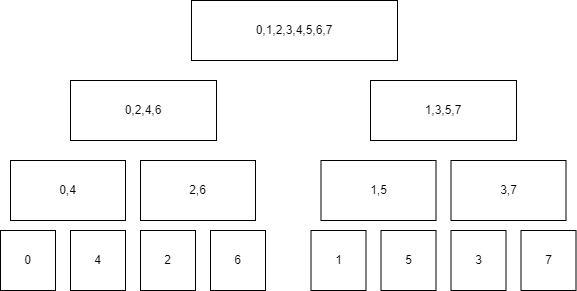
\includegraphics[width=1.2cm]{1.eps}}  %页眉右侧放置logo
\lfoot{}          %页脚左边
\cfoot{\thepage}  %页脚中间
\rfoot{}          %页脚右边

\lstset{
    basicstyle=\small\ttfamily,
    keywordstyle=\color{blue},
    commentstyle=\color{gray!50!black!50},
    backgroundcolor=\color{gray!5},
    stringstyle=\slshape\color{red},
    rulecolor=\color{gray!90},
    breaklines=true,
    frame=leftline,
    numbers=left,
	numberstyle=\footnotesize\itshape,
	firstnumber=1,
	stepnumber=1,
	numbersep=7pt,
}

\begin{document}

\thispagestyle{empty}

\begin{figure}[t]
    \centering
    \includegraphics[width=13cm]{/mnt/d/onedrive/resource/sjtu/logo/LogoChEnUD.png}
\end{figure}

\vspace*{\fill}
\begin{center}
    \Huge\textbf{大整数类 int2048}\\
    \Huge\textbf{算法实现报告}
\end{center}
\vspace*{\fill}

\begin{table}[b]
    \centering
    \large
    \begin{tabular}{ll}
        \textbf{课程:}     & 程序设计 (A类) \\
        \textbf{课程编号:} & CS1953-01      \\
        \textbf{姓名:}     & 潘屹           \\
        \textbf{班级:}     & 电院2231       \\
        \textbf{时间:}     & 2022年11月     \\
        ~                                   \\
        ~                                   \\
        ~                                   \\
        ~                                   \\
        ~                                   \\
        ~                                   \\
    \end{tabular}
\end{table}

\newpage

\thispagestyle{empty}

\section{高精度乘法}

\subsection{多项式}

多项式具有两种常见的表达方式: 点值表达和系数表达. 系数表达是常见的表达方式, 即通过 $n+1$ 个系数给出 $n$ 次多项式的表示. 点值表达则是通过 $n+1$ 个点的横纵坐标来表示出这一多项式函数. 相关基础知识在张驰豪老师第十周伟大思想课程的课堂笔记上已经进行总结, 在此不做展开. 总而言之, 为了得到一个多项式的系数表示, 我们可以先考虑取 $n+1$ 个点进行求值, 再将这些点值转化为系数表达形式, 通过这两个步骤就可以得到原始的多项式.

\subsection{DFT 离散傅里叶变换}

考虑对两个多项式做乘法, 如果运用系数表示法, 显然需要 $O(n^2)$ 的时间复杂度, 而如果已知两个多项式的点值表示法, 则只需要 $O(n)$ 的时间复杂度. 因为只需要将对应的点值纵坐标相乘就可以了.


而求出一个 $n$ 次多项式在每个 $n$ 次单位根下的点值的过程, 被称为离散傅里叶变换(Discrete Fourier Transform, DFT), 而将这些点值重新插值成系数表示法的过程, 叫做离散傅里叶逆变换 (Inverse Discrete Fourier Transform, IDFT).

DFT 的过程即为求出一个长度为 $n$ 数列 $\{b_i\}$, 这个数列的第 $k$ 项为 $A(x)$ 在 $n$ 次单位根的 $k$ 次幂处的点值, 因此有
\begin{align*}
    b_k=\sum_{i = 0}^{n - 1} a_i \times \omega_{n}^i
\end{align*}

IDFT 则是在已知一个 $(n - 1)$ 次多项式 $A(x)=\sum_{i = 0}^{n - 1} a_i x^i$ 进行了离散傅里叶变换后的点值 $\{b_i\}$, 即
\begin{align*}
    b_k=\sum_{i = 0}^{n - 1} a_i \times \omega_n^{ik}
\end{align*}

现在试图还原系数数列 $\{a_i\}$, 推导过程比较复杂, 我们直接给出结论:
\begin{align*}
    a_k=\frac{1}{n} \sum_{i = 0}^{n - 1} b_i \omega_n^{-ki}
\end{align*}

但是我们将一个多项式从系数表示法改为点值表示法需要 $O(n^2)$ 的复杂度 (因为每个横坐标都需要 $O(n)$ 的时间去计算), 而将一个点值表示法改为系数表示法则需要 $O(n^3)$ 的复杂度来做高斯消元. 因此只有我们将这两步都优化至低于 $O(n^2)$ 的复杂度, 才可以得到一个比直接用系数表示法乘更优的做法.

我们考虑使用快速傅里叶变换 (Fast Fourier Transform, FFT)来优化这个过程.

\subsection{FFT 快速傅里叶变换}

我们考虑对 $A(x)$ 按照系数角标的奇偶性分类, 即
\begin{align*}
    A(x)=\sum_{i = 0}^{n - 1} a_i x^i=\sum_{i = 0}^m a_{2i} \times x^{2i} + \sum_{i = 0}^m a_{2i + 1} \times x^{2^i + 1}
\end{align*}
对于上式的后半部分, 提出一个 x, 得到
\begin{align*}
    A(x)=\sum_{i = 0}^{m - 1} a_{2i} x^{i2} + x\sum_{i = 0}^{m - 1} a_{2i + 1} x^{2i}=\sum_{i = 0}^{m - 1} a_{2i} (x^{2})^{i} + x\sum_{i = 0}^{m - 1} a_{2i + 1} (x^2)^{i}
\end{align*}
设 $A_0(x)$ 是一个 $(m-1)$ 次多项式, 满足
\begin{align*}
    A_0(x)=\sum_{i = 0}^{m - 1} a_{2i} x^i
\end{align*}
设 $A_1(x)$ 是一个 $(m-1)$ 次多项式, 满足
\begin{align*}
    A_1(x)=\sum_{i = 0}^{m - 1} a_{2i + 1}x^i
\end{align*}
联立以上三式, 可以得到
\begin{align*}
    A(x)=A_0(x^2) + x \times A_1(x^2)
\end{align*}
对于 $k<\frac{n}{2}$ , 我们有
\begin{align*}
    A(\omega_n^k)=A_0(\omega_n^{2k})+\omega_n^kA_1(\omega_n^{2k})=A_0(\omega_{\frac{n}{2}}^k)+\omega_n^kA_1(\omega_{\frac{n}{2}}^k)
\end{align*}
对于 $k>\frac{n}{2}$, 将次数替换为$k+\frac{n}{2}$, 就有了
\begin{align*}
    A\left(\omega_n^{k+\frac{n}{2}}\right)=A_0\left(\omega_{n}^{2k+n}\right)+\omega_{n}^{k+\frac{n}{2}}A_1(\omega_n^{2k+n})=A_0(\omega_{\frac{n}{2}}^k)-\omega_n^Af_1(\omega_{\frac{n}{2}}^k)
\end{align*}

于是, 大于 $m$ 次的点值可以由 $A_0$ 和 $A_1$ 在小于 $m$ 次的点值求出. 只要求出了 $A_0$ 和 $A_1$ 在小于 $m$ 次的点值, 就可以线性求出 $A$ 在整个 $n$ 次幂处的点值. 而求 $A_0$ 和 $A_1$ 在小于 $m$ 次的点值也是可以递归求解的.

考虑时间复杂度:递推关系为 $T(n)=2T(n / 2) + O(n)$. 因为 $O(n)=\Theta(n)$, 所以 $T(n)=\Theta(n^{\log_2^2} \log n) = \Theta(n \log n)$. 由此, 得到了快速计算 DFT 的办法, 并证明了其时间复杂度为 $O(n \log n)$. 这种方法被即为 FFT.

而对于其逆过程, 也即快速求解
\begin{align*}
    a_k=\frac{1}{n} \sum_{i = 0}^{n - 1} b_i \omega_n^{-ki}
\end{align*}
可以考虑把 $\omega_n^{-k}$ 看做 $n$ 次本原单位根每次逆时针旋转本原单位根幅角的弧度, 因此 $\omega_n^{-k}$ 和 $\omega_n^k$ 是一一对应的. 具体的, $w_n^{-k} = w_n^{k + n}$ . 

因此我们只需要使用 FFT 的方法, 求出 $B(x)$ 在 $\omega_n$ 各个幂次下的值, 然后数组反过来, 即令 $a_k=\frac{1}{n} \sum_{i = 0}^n B(w_n^{n - k})$ 即可. 这一步快速计算插值的过程叫做快速傅里叶逆变换 (Inverse Fast Fourier Transform, IFFT). 

\subsection{递归实现}

\begin{lstlisting}[language=C++]
void FFT(std::vector<complex> &A, int n) {
    if (n == 1)
        return;
    int m = n >> 1;
    std::vector<complex> A0, A1;
    A0.resize(m);
    A1.resize(m);
    for (int i = 0; i < m; ++i) {
        A0[i] = A[i << 1];
        A1[i] = A[(i << 1) | 1];
    }
    FFT(A0, m);
    FFT(A1, m);
    complex w1(cos(Pi / m), sin(Pi / m));
    complex w = std::complex<double>(1.0, 0.0);
    for (int i = 0; i < m; ++i) {
        A[i] = A0[i] + w * A1[i];
        A[i + m] = A0[i] - w * A1[i];
        w *= w1;
    }
}
void IFFT(complex *A, int n) {
  FFT(A, n)
  std::reverse(A + 1, A + n);
}
\end{lstlisting}

\subsection{递推实现}

由于上面的过程递归与动态开空间带来了很大的时间常数, 因此在数据较大时速度较慢, 考虑对其进行优化. 对于 $n=2^3$ 的情况, 我们的操作步骤是这样的.

\begin{figure}[H] 
    \centering
    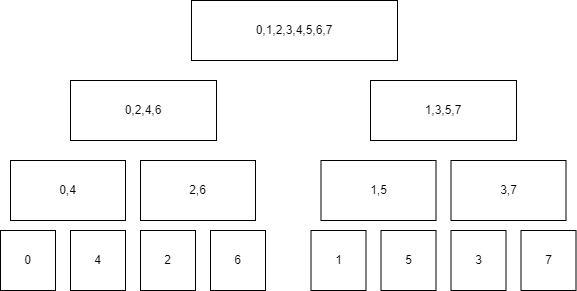
\includegraphics[width=0.8\textwidth]{1.png}
\end{figure}

观察发现, 每个数字与其二进制相反的位置交换. 于是我们只需要先进行 change 操作

\begin{lstlisting}[language=C++]
void change(std::vector<complex> &A, int len) {
    for (int i = 1, j = len / 2; i < len - 1; i++) {
        if (i < j)
            std::swap(A[i], A[j]);
        int k = len / 2;
        while (j >= k) {
            j -= k;
            k >>= 1;
        }
        if (j < k)
            j += k;
    }
}
\end{lstlisting}

\subsection{进位}

这样一来, 就可以把两个大整数相乘的过程看作简单的卷积操作, 最后不要忘记进位!

\begin{lstlisting}[language=C++]
void change(std::vector<complex> &A, int len) {
    for (int i = 1, j = len / 2; i < len - 1; i++) {
        if (i < j)
            std::swap(A[i], A[j]);
        int k = len / 2;
        while (j >= k) {
            j -= k;
            k >>= 1;
        }
        if (j < k)
            j += k;
    }
}
\end{lstlisting}

\section{高精度除法}

\subsection{牛顿迭代法}
对于两个大整数 $a,b$, 设 $n=\left\lfloor\lg a\right\rfloor, m=\left\lfloor\lg b\right\rfloor$ 考虑将他们的除法转化为乘法 $\frac{a}{b}:=a\times\frac{1}{b}$, 右边的 $1/b$ 则可以通过实数求倒数的牛顿迭代方法
\begin{align*}
    x_{n+1}=2x_n-bx_n^2.
\end{align*}
但它的倒数显然是一个浮点数, 因此首先考虑移位, 即将 $\frac{a}{b}$ 转化为 $\left\lfloor\frac{a\left\lfloor\frac{t}{b}\right\rfloor}{t}\right\rfloor$, 这里的 $t=10^p$, 以方便进行移位操作. 对于 $m$ 的选取, 考虑误差分析 
\begin{align*}
\left\lfloor\frac ab\right\rfloor-\left\lceil\frac at\right\rceil\le \left\lfloor\frac ab-\frac at\right\rfloor\le \left\lfloor\frac{a\lfloor\frac tb\rfloor}t\right\rfloor\le \left\lfloor\frac ab\right\rfloor
\end{align*}
因此 $\left\lfloor\frac{a\lfloor\frac tb\rfloor}t\right\rfloor$ 与答案的差不大于 $\left\lceil\frac{a}{t}\right\rceil$, 只需取 $p=n\ge\lg a$ 就能保证误差不大于 $1$, 这样的误差可以最后进行调整. 特殊地, 若 $n>2m$, 可以将 $a,b$ 同时乘以 $g^{n-2m}$ 使得 $n'\le 2m'$, 因此只需求出 $\left\lfloor\frac {g^{2m}}b\right\rfloor$.

实现过程如下, 其中 inv() 部分在下一节中讲解.

\begin{lstlisting}[language=C++]
int2048 &int2048::operator/=(int2048 num_right) {
    if (*this < num_right)
        return *this = 0;
    int2048 num_left = *this;
    int len_left = num_left.num.size(), len_right = num_right.num.size();
    if (len_left > len_right * 2) {
        int len_move = len_left - len_right * 2;
        num_left.move_digit(len_move);
        num_right.move_digit(len_move);
        len_right += len_move;
        len_left -= len_move;
    }
    int2048 inv_num_right = num_right.inv();
    int2048 res = len_left * inv_num_right;
    res.move_digit(-(len_right * 2));
    modify(*this, num_right, res);
    res.reduce();
    return *this = res;
}
\end{lstlisting}

\subsection{求逆与误差分析}
下面的问题就是求解 $\left\lfloor\frac{10^{2m}}{b}\right\rfloor$. 设在前一次迭代中, 已求出 $b$ 的最高 $k$ 位的答案. 形式化地说, 设 $c=\frac {g^{2m}}b$, 已知 $b'=\left\lfloor\frac{b}{g^{m-k}}\right\rfloor,c'=\left\lfloor\frac {g^{2k}}{b'}\right\rfloor$, 要求 $\lfloor c\rfloor$. 那么迭代容易得到
\begin{align*}
    c^*=2c'g^{m-k}-bc'^2g^{-2k}
\end{align*}
作为 $c$ 的近似值.

根据误差分析\footnote{倪泽堃, 理性愉悦: 高精度数值计算, 2012 年 NOI 冬令营}以及该结论在 $g$ 进制下的推广\footnote{https://www.luogu.com.cn/blog/88403/solution-p5432}, 最终的迭代结果误差不超过 $2g^{m-2k+3}$. 因此, 取 $k=\left\lfloor\frac{m}{2}\right\rfloor+2$, 则有误差 $\Delta\le 2g^{-1}<1$, 同样至多只需要调整一次. 至于递归次数, 因为每次 $k\le \frac{m+5}2$, 所以递归 $x$ 次后 $m'$ 不超过 $\frac{m}{2^x}+5$, 可以当 $m\le 10$ 时使用暴力除法. 

实现过程如下. 显然, 全过程的时间复杂度为 $O(n\log n)$.

\begin{lstlisting}[language=C++]
int2048 int2048::inv() {
    if (num.size() <= 10) {
        int2048 res;
        int siz = num.size() << 1 | 1;
        res.num.resize(siz);
        res.num[res.num.size() - 1] = 1;
        res.div(*this);
        return res;
    } else {
        int2048 pre, inv_pre;
        int len = num.size(), pre_len = (num.size() + 5) >> 1;
        pre.num.clear();
        pre.num.resize(pre_len);
        for (int i = pre_len - 1, j = len - 1; i >= 0; i--, j--)
            pre.num[i] = num[j];
        inv_pre = pre.inv();
        int2048 part1 = *this * inv_pre * inv_pre;
        part1.move_digit(-2 * pre_len);
        int2048 part2 = 2 * inv_pre;
        part2.move_digit(len - pre_len);
        int2048 res = part1 - part2 - 1;
        int2048 num_one;
        num_one.num.clear();
        num_one.num.resize(len << 1 | 1);
        num_one.num[len << 1] = 1;
        modify(num_one, *this, res);
        res.reduce();
        return res;
    }
}
\end{lstlisting}

\end{document}